\chapter[转动动力学]{\itr{Rotation Dynamics}{转动动力学}}
\begin{solution}[{\large\color{plainred}Determine the Moment of Inertia of an Irregularly Shaped Object}\\
	This problem describes one experimental method of
	determining the moment of inertia of an irregularly
	shaped object such as the \itr{payload}{有效负载} for a satellite. \\
	The figure shows a mass $m$ \itr{suspended}{悬挂} by a \itr{cord}{绳子} \itr{wound}{被缠绕}
	around a spool of radius $r$, forming part of a \itr{turntable}{转台}
	supporting the object. When the mass is released from
	rest, it \itr{descends}{下降} through a distance $h$, acquiring a speed
	$\vec{v}$. Show that the moment of inertia $I$ of the equipment
	(including the turntable) is\quad$mr^2(\dfrac{2gh}{v^2}-1)$. ]
	\begin{center}
		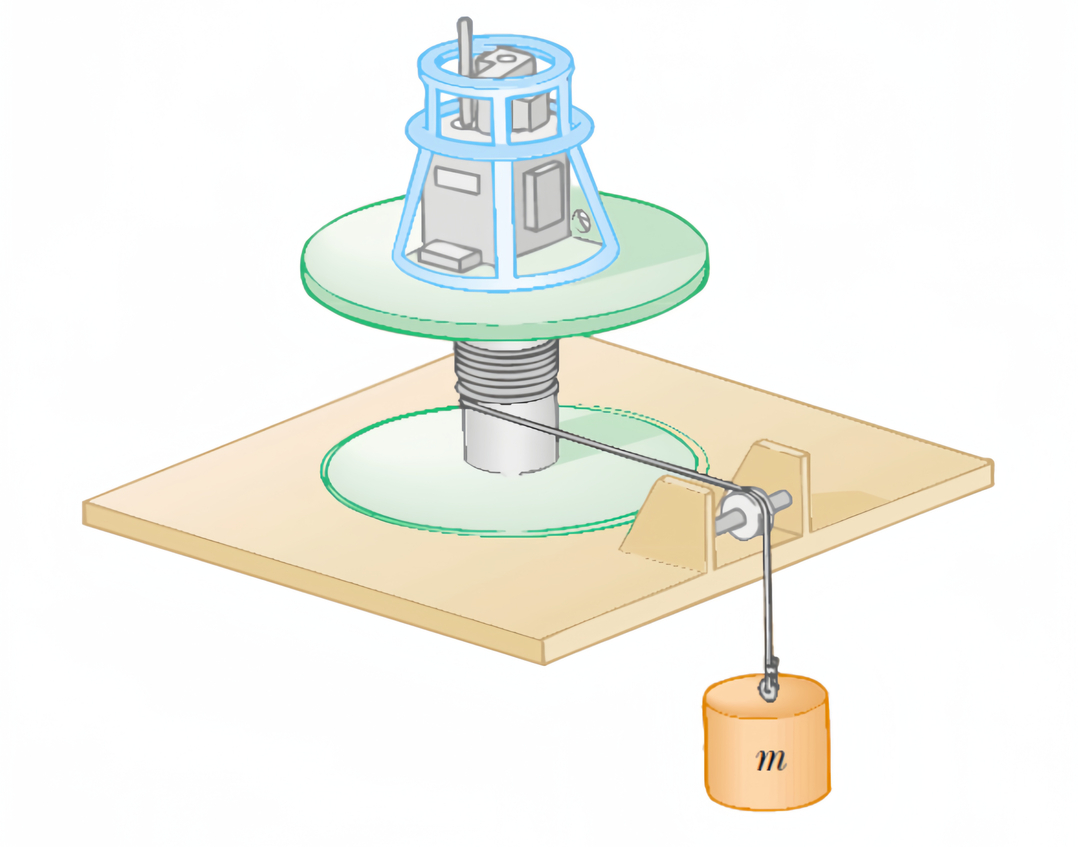
\includegraphics[width=0.6\textwidth]{chapter3_example_1}
	\end{center}
	
	这是一道基础的转动力学题目,一般的求解思路为:列力学方程---列运动方程---列关联方程---求解。
	
	设绳子的张力为$\vec{T}$,物体的转动惯量为$I$,有:
	\[\left\{
		\begin{array}{cc}
			\left.\begin{array}{c}
				Tr=I\alpha\\
				mg-T=ma
			\end{array}\right\}&\cdots\text{力学方程}\\
			v^2=2ah&\cdots\text{运动方程}\\
			a=r\alpha&\cdots\text{关联方程}
		\end{array}
		\right.\]
	联立求解即得\[I=mr^2(\dfrac{2gh}{v^2}-1)\]
\end{solution}
\begin{solution}[{\large\color{plainred}Rolling Items}\\
	Three objects of \itr{uniform density}{均匀的密度} --- a \itr{solid sphere}{实心球}, a \itr{solid
		cylinder}{实心圆柱}, and a \itr{hollow cylinder}{空心圆柱} --- are placed at the top of
	an \itr{incline}{斜坡}. \\
	If they all are released from rest
	at the same \itr{elevation}{高度} and roll without \itr{slipping}{滑动}, which object reaches the bottom first?
	]
	\begin{center}
		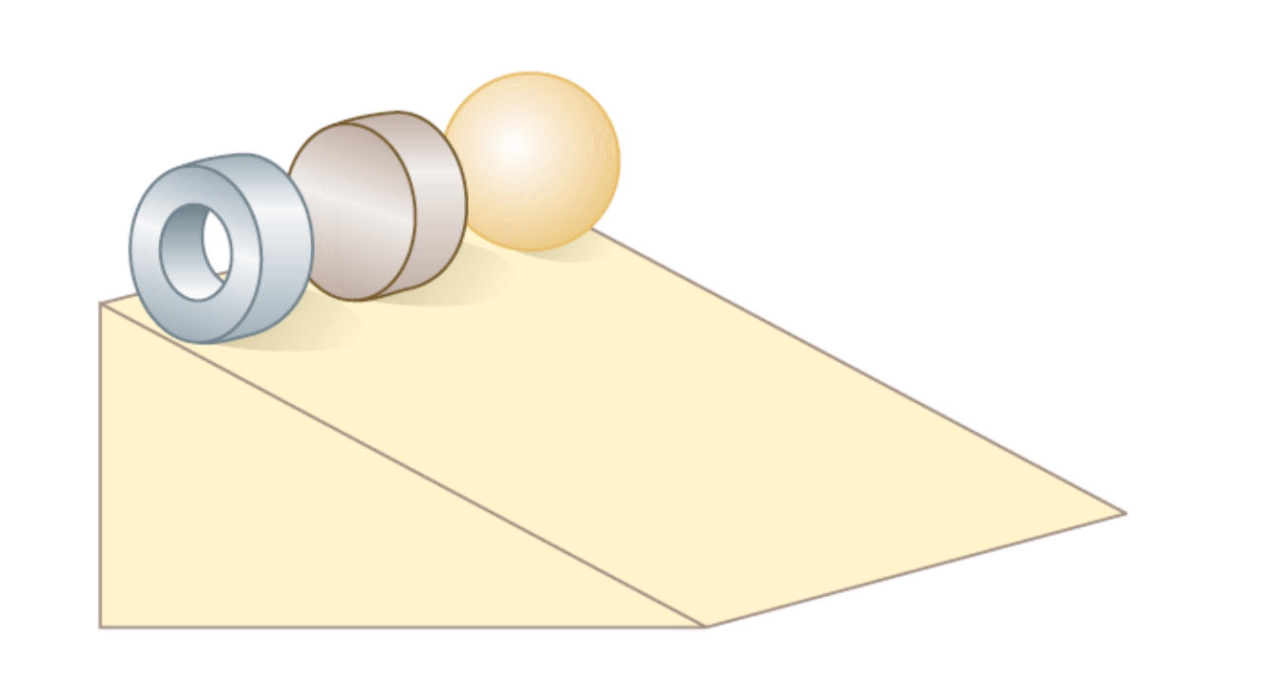
\includegraphics[width=0.6\textwidth]{chapter3_example_2}
	\end{center}
	
	本题是经典的纯滚动问题。所谓纯滚动,就是滚动体与接触面接触的点速度为$\vec{0}$(即旋转速度和质心速度相抵消)。
	%分析纯滚动时,我们往往以接触线为转动轴,以避免引入非惯性系,将问题复杂化。
	
	我们往往选择过质心的轴作为旋转轴,建立参考系。这是因为,即使这样建立的参考系是一个非惯性系,只要它不发生转动,那么,使用证明“均匀重力场中重力可以等效作用在质心”中用到的方法(\refleaftext{prove3.7}),就可以证明惯性力可以等效作用在质心。由于我们选择的是质心轴,惯性力产生的力矩恒为$0$,因此也就不会对转动的分析产生影响\footnote{很多解析都直接选择了一个非惯性质心系来分析转动,却并没有讲解惯性力可以忽略的原因。}。
	
	现在,让我们选择质心系分析问题\footnote{当然,过质心的轴有很多,但是大家应该能意会到选择了怎样的轴(对称性好的轴),就不再描述了}。
	
	若记球体$m_1$的转动惯量为$I_1$,实心圆柱$m_2$的转动惯量为$I_2$,空心圆柱$m_3$的转动惯量为$I_3$,斜面倾角为$\theta$,则有:
	\[\left\{
		\begin{array}{l}
			m_1a_1=m_1g\sin\theta-f_1\\
			m_2a_2=m_2g\sin\theta-f_2\\
			m_3a_3=m_3g\sin\theta-f_3\\
			 f_1r_1=I_1\alpha_1\\
			 f_2r_2=I_2\alpha_2\\
			 f_3r_3=I_3\alpha_3\\
			a_1=r_1\alpha_1\\
			a_2=r_2\alpha_2\\
			a_3=r_3\alpha_3
		\end{array}
	\right.\]
	于是解得
	\[\left\{
		\begin{array}{l}
			a_1=\dfrac{m_1r_1{}^2}{I_1+m_1r_1{}^2}g\sin\theta\\[2ex]
			a_2=\dfrac{m_2r_2{}^2}{I_2+m_2r_2{}^2}g\sin\theta\\[2ex]
			a_3=\dfrac{m_3r_3{}^2}{I_3+m_3r_3{}^2}g\sin\theta
		\end{array}
	\right.\]
	由常见物体的转动惯量(见\refleaftext{chapter3_moment_inertia2})知
	\begin{align*}
		I_1&=\dfrac{2}{5}m_1r_1{}^2\\
		I_2&=\dfrac{1}{2}m_2r_2{}^2\\
		I_3&=\dfrac{1}{2}m_3(r_{3(inner)}{}^2+r_3{}^2)
	\end{align*}
	易知
	\[a_1>a_2>a_3\]
	故实心球快于实心圆柱快于空心圆柱。
\end{solution}
%\refleaf*{law3.1}[-40ex]
%\refleaf*{chapter3_moment_inertia2}[-35.6ex]
\newpage
\begin{solution}[\En{\large Calculation of the Moment of Inertia}\\A rod's \itr{linear density}{线密度} is given by $\lambda=kx$, where $x$ represents the distance from the point to the rod's center. \\
	Given the length of the rod $l$, try to calculate the moment of inertia of the rod, given the rotation axis at:\\	
	(1) Center $O$ as the $y$ axis shows.\\
	(2) One end as the $y'$ axis shows.]
	\ctikzfig{chapter3_example_3_3}
	(1)由于$O$也是质心位置,不妨先求$I_{CM}$,再利用平行轴定理求解$I_{end}$。
	注意到
	\[\dif m=\lambda\dif x=k|x|\dif x\]
	于是
	\begin{align*}
		\int_{-\frac{L}{2}}^{\frac{L}{2}}(x^2)(k|x|)\dif x&=2\int_0^{\frac{L}{2}}kx^3\dif x\\
		&=2\left.(\dfrac{1}{4}kx^4)\right|_0^{\frac{L}{2}}\\
		&=\dfrac{1}{32}kL^4
	\end{align*}
	
	(2)欲用平行轴定理(\refleaftext{law3.1}),则需知晓棍子的质量。
	\begin{align*}
		m&=\int_{-\frac{L}{2}}^{\frac{L}{2}}k|x|\dif x\\
		&=2\int_0^{\frac{L}{2}}kx\dif x\\
		&=2\left.(\dfrac{1}{2}kx^2)\right|_0^{\frac{L}{2}}\\
		&=\dfrac{1}{4}kL^2
	\end{align*}
	故
	\[I_{end}=I_{CM}+m(\dfrac{L}{2})^2=\dfrac{3}{32}kL^4\]
\end{solution}
\begin{solution}[\En{\large Massive \itr{Pulley}{滑轮}}\\Consider two \itr{cylinders}{圆柱} having masses $m_1$
	and $m_2$, where $m_1 < m_2$, connected by a
	string passing over a pulley. The pulley
	has a radius $R$ and moment of inertia $I$
	about its axis of rotation. The string does
	not \itr{slip}{滑动} on the pulley, and the system
	is released from rest. Find the linear
	speeds of the cylinders after
	cylinder 2 \itr{descends}{下降} through a
	distance $h$, and the angular
	speed $\omega$ of the pulley at this time.]
	\begin{center}
		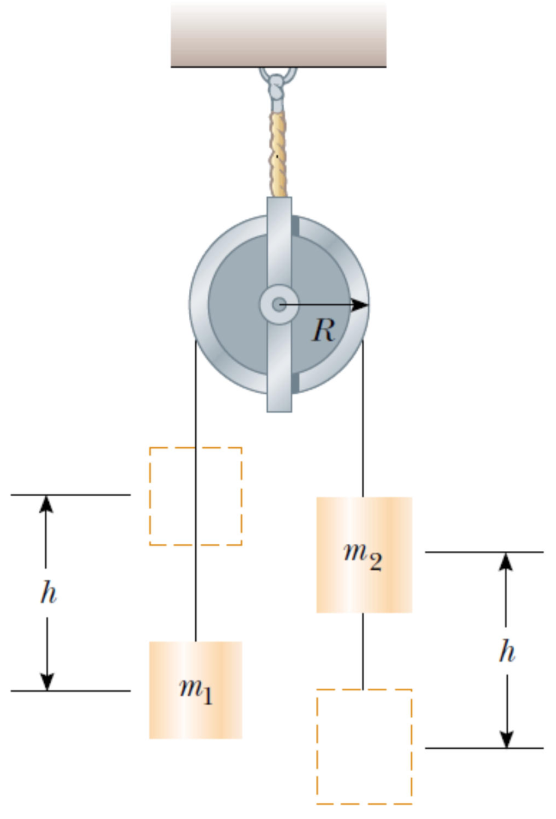
\includegraphics[width=0.3\textwidth]{chapter3_massive_pulley}
	\end{center}
	本题可从运动角度或能量角度考虑。\\
	法一:运动分析\\
	设左绳的张力为$T_1$,右绳的张力为$T_2$,则有
	\[\left\{\begin{array}{c}
		T_1-m_1g=m_1a\\
		T_2R-T_1R=I\alpha\\
		m_2g-T_2=m_2a\\
		a=R\alpha
	\end{array}\right.\]
	于是解得
	\[a=\dfrac{m_2-m_1}{m_1+m_2+\frac{I}{R^2}}g\]
	则
	\[v=\sqrt{2ah}=\sqrt{\dfrac{m_2-m_1}{m_1+m_2+\frac{I}{R^2}}2gh},\quad\omega=\sqrt{\dfrac{m_2-m_1}{(m_1+m_2)R^2+I}2gh}\]
	法二:能量分析\\
	系统机械能守恒,于是有
	\[\left\{\begin{array}{c}
		m_2gh=m_1gh+\dfrac{1}{2}m_1v^2+\dfrac{1}{2}m_2v^2+\dfrac{1}{2}I\omega^2\\
		v=R\omega
	\end{array}\right.\]
	亦可解得
	\[v=\sqrt{2ah}=\sqrt{\dfrac{m_2-m_1}{m_1+m_2+\frac{I}{R^2}}2gh},\quad\omega=\sqrt{\dfrac{m_2-m_1}{(m_1+m_2)R^2+I}2gh}\]
\end{solution}
\begin{solution}[\En{\large Object rotating on a string
		of changing length}\\Initially, the mass \itr{revolves}{转动} with a speed $v_1$ = 2.4 m/s in
		a circle of radius $R_1$ = 0.80 m.
		The string is then pulled slowly through the hole so
		that the radius is reduced to $R_2$ = 0.48 m. What is the
		speed, $v_2$, of the mass now?]
	\begin{center}
		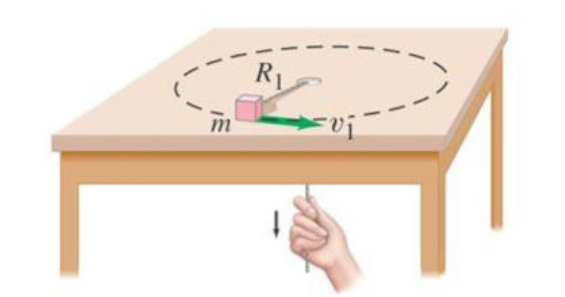
\includegraphics[width=0.7\textwidth]{chapter3_string}
	\end{center}
	本题考察角动量守恒。可以注意到,绳子对物块的力始终是径向的,对应的力矩始终为$\vec{0}$,因此,物块的角动量守恒。不妨就以洞为轴,有
	\[I_1\omega_1=I_2\omega_2\Rightarrow R_1{}^2\omega_1=R_2{}^2\omega_2\]
	代入$\omega_1=\dfrac{v_1}{R_1},\quad\omega_2=\dfrac{v_2}{R_2}$,即得
	\[v_1R_1=v_2R_2\]
	代入数据即得$v_2=4.0$m/s.
\end{solution}
\begin{solution}[\En{\large Rotation of a sliding rigid rod}\\Consider a rod with mass m and length L standing straight on the friction-less ground. When we
	release the rod, it will fall from the unstable \itr{equilibrium position}{平衡位置}\!.\\
	(a) Calculate the angular velocity of the rod, when it has an angle of $\theta$ with respect to the ground
	as illustrated in Figure 1.\\
	(b) What is the final angular velocity $\omega_1$ of the rod before it hits the ground?\\
	(c) If the same rod is leaning to a frictionless wall with an initial angle of α to the frictionless
	ground (see Figure 2), what is the final angular velocity $\omega_2$ of the rod before it hits the ground?\\
	{\em Note that there is a possibility that the right end of the rod leaves from the wall before the rod hits the ground.}]
	\begin{center}
		\begin{minipage}{0.45\textwidth}
			\centering
			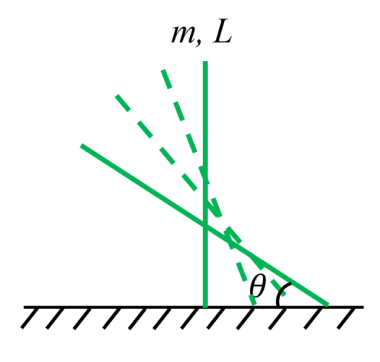
\includegraphics[width=\linewidth]{chapter3_rotating_rod_1}\\
			Figure 1
		\end{minipage}
		\quad
		\begin{minipage}{0.45\textwidth}
			\centering
			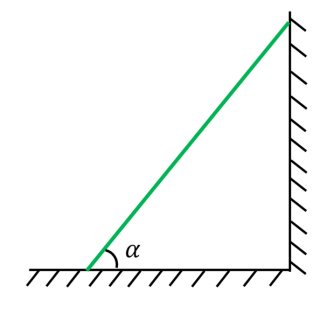
\includegraphics[width=\linewidth]{chapter3_rotating_rod_2}\\
			Figure 2
		\end{minipage}
	\end{center}
	本题主要考察转动中的能量守恒,以及对平动速度和角速度关系的分析。
	
	(a) 首先,由题意知不存在摩擦力,而支持力做功始终为零,所以以棍子为研究对象,有机械能守恒。又注意到,棍子在水平方向始终不受力,因此质心是在垂直下降。于是有
	\begin{equation}
		mg\dfrac{L}{2}-mg\dfrac{L}{2}\sin\theta=\dfrac{1}{2}mv_{_{CM}}{}^2+\dfrac{1}{2}I\omega^2
	\end{equation}
	研究质心的运动,有
	\begin{align}
		v_{_{CM}}&=\dfrac{\dif (\dfrac{L}{2}\sin\theta)}{\dif t}\\[1ex]
		&=\dfrac{L}{2}\dfrac{\dif\sin\theta}{\dif\theta}\dfrac{\dif\theta}{\dif t}\\[1ex]
		&=\dfrac{L}{2}\cos\theta\omega
	\end{align}
	将(3.4)代入(3.1)即得
	\begin{equation}
		\omega=2\sqrt{\dfrac{3g}{L}\dfrac{1-\sin\theta}{1+3\cos^2\theta}}
	\end{equation}
	(b) 即考虑(a)中的极限情况,将$\theta=0$代入(3.5)中即得
	\begin{equation}
		\omega_1=\sqrt{\dfrac{3g}{L}}
	\end{equation}
	(c) \begin{center}
		\begin{tikzpicture}[scale=2]
			\coordinate (O) at (0,0);  
			\coordinate (A) at (-1,0);  
			\coordinate (B) at (0,1.732); 
			\coordinate (D) at (-1.5,0);
			\coordinate (E) at (0,2.5); 
			\coordinate (BB) at (0,1.414);
			\coordinate (AA) at (-1.414,0);
			
			\draw [green](A) -- (B) ; 
			\draw [thick=3pt](D)--(O);
			\draw [thick=3pt](O)--(E);
			\draw [green,dashed](AA)--(BB);
			
			\coordinate (M) at ($(A)!0.5!(B)$);  
			\coordinate (N) at ($(AA)!0.5!(BB)$);
			
			\draw[dashed,plainred] (O) -- (M);  
			\draw[dashed,plainred] (O)--(N);
			\draw[dashed,yellow5] (0,0) circle[radius=1];
			
			\node[below left] at (A) {$A$};  
			\node[above right] at (B) {$B$};  
			\node[above right] at (BB) {$B'$};
			\node[below left] at(AA) {$A'$};
			\node[above left] at (M) {$C$};  
			\node[below left] at (O) {$O$};  
			\node[above right]at (A) {$\ \ \ \alpha$};
			\node[above left] at (N) {$C'$};
			\draw (-0.8,0) arc(0:60:0.2);
			\draw (-1.214,0) arc (0:45:0.2);
			\node[above right] at (AA) {$\ \ \ \,\theta$};
		\end{tikzpicture}  
	\end{center}
		
如图,先考虑棍未与墙壁脱离情形,注意到质心$C$到$O$的距离始终为$\dfrac{L}{2}$,因此确定质心的运动轨迹是一个圆。由$\angle COA=\angle CAO$,知$v_{_{CM}}=\omega\dfrac{L}{2}$,即关系式。再由\\[1ex]“无摩擦力”,“支持力不做功”知棍子机械能守恒,于是可以列出守恒式:
		\begin{equation}
			mg(\dfrac{L}{2}\sin\alpha-\dfrac{L}{2}\sin\theta)=\dfrac{1}{2}mv_{_{CM}}{}^2+\dfrac{1}{2}I\omega^2
		\end{equation}
由(3.7)可解得
\begin{equation}
	\omega=\sqrt{\dfrac{3g(\sin\alpha-\sin\theta)}{L}}
\end{equation}
接下来,我们考虑临界条件。当棍子脱离墙时,来自墙的支持力消失,也就是说,\textbf{质心在水平方向不再拥有加速度}。于是,$v_{_{CM}x}$最大时,棍子将脱离墙。
\begin{align}
	v_{_{CM}x}&=v_{_{CM}}\sin\theta\\
	&=\omega\dfrac{L}{2}\sin\theta\\
	&=\dfrac{\sin\theta}{2}\sqrt{3gL(\sin\alpha-\sin\theta)}\\
	&=\sqrt{3gL}\cdot\sqrt{\dfrac{\sin\theta}{2}}\cdot\sqrt{\dfrac{\sin\theta}{2}}\cdot\sqrt{\sin\alpha-\sin\theta}\\
	&\le\dfrac{1}{3}\sin\alpha\sqrt{gL\sin\alpha}\quad(\text{当且仅当}\sin\theta=\dfrac{2}{3}\sin\alpha)
\end{align}
之后,在水平方向,质心的运动保持不变。由(3.4)知,当棍子即将落地时,有\begin{equation}
	v_{_{CM}y}=\dfrac{L}{2}\omega_2
\end{equation}于是可以列守恒式
\begin{equation}
	mg\dfrac{L}{2}\sin\alpha=\dfrac{1}{2}m(v_{_{CM}x}{}^2+v_{_{CM}y}{}^2)+\dfrac{1}{2}I\omega_2{}^2
\end{equation}
将(3.14)代入(3.15)即得
\begin{equation}
	\omega_2=\sqrt{(9\sin\alpha-\sin^3\alpha)\dfrac{g}{3L}}
\end{equation}
\dove\ PS:这大概是本章考察的天花板了。
\end{solution}
